\documentclass{article}
\usepackage{amsthm}
\usepackage{comment}
\usepackage{amsmath}
\usepackage{amsfonts}
\usepackage{sectsty}
\usepackage{hyperref}
\usepackage{fancyhdr}
\usepackage[top=1in,bottom=1in,left=1in,right=1in]{geometry}
\usepackage{float}
\usepackage{graphicx}
\usepackage{tabularx}
\usepackage{mathtools}

\newtheorem{theorem}{Theorem}

\title{Lecture 2 - Induction and Cardinality}
\author{Matthew Farah, \href{mailto:farahm11@mcmaster.ca}{$\langle$farahm11@mcmaster.ca$\rangle$}, 400468251}
\date{\today}

\hypersetup{
        colorlinks=true,
        linkcolor=blue,
        filecolor=magenta,
        urlcolor=blue,
        citecolor=blue,
	anchorcolor=blue
}

\fancyhead{}
\fancyhead[L]{Matthew Farah, \href{mailto:farahm11@mcmaster.ca}{$\langle$farahm11@mcmaster.ca$\rangle$}, 400468251}
\fancyhead[R]{Lecture 2 - Induction and Cardinality}

\newenvironment{directsubsubs}{
  \makeatletter
  \renewcommand\thesubsubsection{\thesection.\Roman{subsubsection}}
  \makeatother
}{
  \makeatletter
  \renewcommand\thesubsubsection{\thesubsection.\Roman{subsubsection}}
  \makeatother
}

\renewcommand{\thesubsection}{\thesection.\alph{subsection}}
\renewcommand{\thesubsubsection}{\thesection.\alph{subsection}.\Roman{subsubsection}}
\makeatletter

\sectionfont{\fontsize{12}{12}\bfseries}
\subsectionfont{\fontsize{10}{12}\normalfont}
\subsubsectionfont{\fontsize{10}{12}\normalfont}

\begin{document}

\maketitle
\pagestyle{fancy}

\begin{itemize}
	\item A natural number n, is a whole number which is greater than or equal to 1.
	\begin{itemize}
		\item Denoted $n \in \mathbb{N}$.
	\end{itemize}
	\item The principle of mathematical induction (or just induction) is used to prove statements about all natural numbers.
	\begin{itemize}
		\item Induction can be given in two formulations:
		\begin{enumerate}
			\item The set formulation of the principle of mathematical induction.
			\item The statement formulation of the principle of mathematical induction.
		\end{enumerate}
		\item Note that induction only works on sets with the well-ordering property.
	\end{itemize}
	\item A statement $P(n)$ about a natural number n is an expression which can either be true or false.
	\begin{itemize}
		\item The statement formulation of induction says that, for some hypothesis about natural numbers $P(n)$, that if some base case $P(b)$ is true, and that $\forall k \in \mathbb{N}, \; k \ge b, P(k) \implies P(k + 1)$, then $P(n)$ must be true for all $\forall n \in \mathbb{N}, n \ge b$.
	\end{itemize}
\end{itemize}

\section[Example ~\thesection]{Prove that the statement $P(n): 1 + 2 + 3 \ldots + n = \frac{(n)(n + 1)}{2}$ is true $\forall n \in \mathbb{N}$ by induction.}

\begin{proof}

We do this in 3 steps: \\

\begin{center}
	\large{\underline{(1) Prove the base case (Show $P(1)$ is true).}}
\end{center}

\vspace{.3cm}

\begin{align*}
	&\text{LHS:}& &\text{RHS:} \\
	&=1 & &=1\frac{(1)(1 + 1)}{1} \\
	&=1 & &=1 \\
\end{align*}

Therefore, $P(1)$ is true. \\

\begin{center}
	\large{\underline{(2) Formulate our induction hypothesis (State $P(k)$).}}
\end{center}

\vspace{.3cm}

Here, we assume that our statement holds true for some $k \in \mathbb{N}$. Therefore, our induction hypothesis can be formulated as:

\begin{align*}
	P(k): 1 + 2 + \ldots + k = \frac{k(k + 1)}{2} \\
\end{align*}

\begin{center}
	\large{\underline{(3) Prove $P(k) \implies P(k + 1)$}} \\
\end{center}

\vspace{.3cm}

\begin{align*}
	&\text{LHS:}& &\text{RHS} \\
	&= 1 + 2 + \ldots + k + k + 1& &=\frac{(k + 1)(k + 2)}{2} \\
	&= \frac{(k)(k + 1)}{2} + k + 1& & \\
	&= \frac{(k)(k + 1)}{2} + \frac{2k + 2}{2}& & \\
	&= \frac{k^2 + k + 2k + 2}{2}& & \\
	&= \frac{k^2 + 3k + 2}{2}& & \\
	&= \frac{(k + 1)(k + 2)}{2}& & \\
\end{align*}

Therefore, since the $LHS = RHS$, we know that $P(k) \implies P(k + 1)$. Since $P(1)$ is true, then $P(1) \implies P(2) \implies \ldots P(n)$ and thus the statement $P(n)$ holds for all $n \in \mathbb{N}$ by principle of mathematical induction.

\end{proof}

\section[Example ~\thesection]{Prove that $1 + r + r^2 + \ldots + r^n = \frac{1 - r^{n + 1}}{1 - r}, r \in \mathbb{R}, n \in \mathbb{N}, r \ne 1$}

\begin{proof}

We formulate our proof as before, first by fixing $r \ne 1$ and defining our statement as $P(n): 1 + r + r^2 + \ldots + r^n = \frac{1 - r^{n - 1}}{1 - r}$. \\

\begin{center}
	\large{\underline{(1) Prove the base case (Show $P(1)$ is true).}}
\end{center}

\vspace{.3cm}

\begin{align*}
	&\text{LHS:}& &\text{RHS:} \\
	&1 + \ldots + r^n& &\frac{1 - r^{n + 1}}{1 - r} \\
	&=1 + r& &=\frac{1 - r^{1 + 1}}{1 - r} \\
	& & &=\frac{1 - r^{2}}{1 - r} \\
	& & &=\frac{(1 + r)(1 - r)}{1 - r} \\
	& & &=1 + r \\
\end{align*}

Therefore, $P(1)$ is true. \\

\begin{center}
	\large{\underline{(2) Formulate our induction hypothesis (State $P(k)$).}}
\end{center}

Here, we assume that our statement holds true for some $k \in \mathbb{N}$. Therefore, our induction hypothesis can be formulated as:

\begin{align*}
	P(k): 1 + r + \ldots + r^k &= \frac{1 - r^{k + 1}}{1 - r} \\
\end{align*}

\begin{center}
	\large{\underline{(3) Prove $P(k) \implies P(k + 1)$}}
\end{center}

Here, as opposed to trying to show the $LHS = RHS$, I'll instead just show that $1 + r + \ldots + r^k + r^{k + 1} = \frac{1 - r^{k + 2}}{1 - r}$ using our induction hypothesis.

\begin{align*}
	&1 + r + \ldots + r^k + r^{k + 1} \\
	&= \frac{1 - r^{k + 1}}{1 - r} + r^{k + 1} \\
	&= \frac{1 - r^{k + 1}}{1 - r} + \frac{(1 - r)r^{k + 1}}{1 - r} \\
	&=\frac{1 - r^{k + 1} + r^{k + 1} - r^{k + 2}}{1 - r} \\
\end{align*}

Therefore, $P(k) \implies P(k + 1)$. Since $P(1)$ is true, then $P(1) \implies P(2) \implies \ldots P(n)$ and thus the statement $P(n)$ holds for all $n \in \mathbb{N}$ by principle of mathematical induction.

\end{proof}

\begin{itemize}
	\item The principle of strong mathematical induction is another technique used to prove statements about the natural numbers.
	\begin{itemize}
		\item In the principle of strong induction, rather than assuming that $P(k)$ holds for some $k \in \mathbb{N}$, we instead assume $P(1) \wedge P(2) \wedge \ldots \wedge P(k)$ and attempt to prove that $P(1) \wedge P(2) \wedge \ldots \wedge P(k) \implies P(k + 1)$.
	\end{itemize}
\end{itemize}

\section[Example ~\thesection]{Suppose $(x_n)$ is a sequence, $x_n \in \mathbb{Q} \; \forall n \in \mathbb{N}$ and $(x_n)$ is defined as $x_1 = 1, x_2 = 2$, and $x_n = \frac{x_{n - 1} + x_{n - 2}}{2}$. Prove that $1 \le x_n \le 2 \; \forall n \in \mathbb{N}$ by strong induction.}

Let $P(n): 1 \le x_n \le 2$.

\begin{center}
	\large{\underline{(1) Prove the base case.}}
\end{center}

\vspace{.3cm}

Since we are dealing with strong mathematical induction, as you will see in our final step of the proof, we need to be sure that \underline{both} $P(1)$ and $P(2)$ hold true. Thankfully, both statements are trivially true.

\begin{align*}
	x_1 &= 1 \\
	x_2 &= 2 \\
\end{align*}

Therefore, since $1 \le x_1 \le 2$ and $1 \le x_2 \le 2$, $P(1)$ and $P(2)$ both hold.

\begin{center}
	\large{\underline{(2) Formulate our induction hypothesis (State $P(k)$).}}
\end{center}

\vspace{.3cm}

Since we are attempting to prove our statement by strong induction, we assume that there exists some $k \in \mathbb{N}$ such that $P(1) \wedge P(2) \wedge \ldots \wedge P(k)$ is true. Therefore, our induction hypothesis is given by:

\begin{align*}
	1 \le x_1 \le 2 \wedge 1 \le x_2 \le 2 \wedge \ldots \wedge 1 \le x_k \le 2 \\
\end{align*}

\begin{center}
	\large{\underline{(3) Prove $P(1) \wedge P(2) \wedge \ldots \wedge P(k) \implies P(k + 1)$}} \\
\end{center}

\vspace{.3cm}

$P(k + 1)$ is the statement $1 \le \frac{x_{k + 1}} \le 2$. By the definition of $(x_n)$, we know that $x_{k + 1} = \frac{x_k + x_{k - 1}}{2}$. Now since we are assuming $P(k - 1) and P(k)$, we assume that $1 \le x_{k - 1} \le 2$ and $1 \le x_k \le 2$, and therefore:

\begin{align*}
	x_{k + 1} = \frac{x_{k} + x_{k - 1}}{2} \implies \quad
\end{align*}
\vspace{-.7cm}
\begin{align*}
	\frac{1 + 1}{2} &\le \frac{x_k + x_{k - 1}}{2} \le \frac{2 + 2}{2} \\
	\frac{2}{2} &\le \frac{x_k + x_{k - 1}}{2} \le \frac{4}{2} \\
	1 &\le \frac{x_k + x_{k - 1}}{2} \le 2
\end{align*}

Therefore, $P(1) \wedge P(2) \wedge \ldots \wedge P(k) \implies P(k + 1)$. Thus, since $P(1)$ and $P(2)$ holds, then by principle of strong mathematical induction, $P(n)$ holds $\forall n \in \mathbb{N}$.

\begin{itemize}
	\item A function $f: A \rightarrow B$ denotes that a function has domain $A$ and co-domain $B$.
	\begin{itemize}
		\item $f$ is a \emph{surjective} (onto) function if $\forall b \in B, \; \exists a \in A$ such that $f(a) = b$.
		\item $f$ is an \emph{injective} (1 to 1) function if $\forall a_1, a_2 \in A, \; a_1 \neq a_2, \; f(a_1) \neq f(a_2)$.
		\item $f$ is \emph{bijective} if it is both injective and surjective.
	\end{itemize}
	\item The set $\mathbb{N}_n$ denotes the first $n$ natural numbers.
	\item The cardinality of a set represents the size of a set.
	\item A set can be either \emph{finite} or \emph{infinite}.
	\begin{itemize}
		\item A set $S$ is finite if it is either the empty set $\emptyset$ or if there exists a bijection between $S$ and $\mathbb{N}_n$ for some unique $n \in \mathbb{N}$.
		\begin{itemize}
			\item $S$ has a cardinality of 0 if $S$ = $\emptyset$ or $n$ for the bijection between $S$ and $\mathbb{N}_n$.
			\item The cardinality of a finite set is denoted $\#S$.
		\end{itemize}
		\item A set S is infinite if there exists no bijection between $S$ and $\mathbb{N}_n \; \forall n \in \mathbb{N}$.
		\begin{itemize}
			\item An infinite set can be either \emph{denumerable} or \emph{uncountable}.
			\begin{itemize}
				\item A set is denumerable if there exists a bijection between $\mathbb{N}$ and $S$.
				\item A set is uncountable if there exists no bijection between $\mathbb{N}$ and $S$.
			\end{itemize}
			\item A set is \emph{Countable} if it is either finite or denumerable.
		\end{itemize}
	\end{itemize}
\end{itemize}

We can visually represent the different kinds of sets with the following Venn diagram:

\begin{figure}[H]
	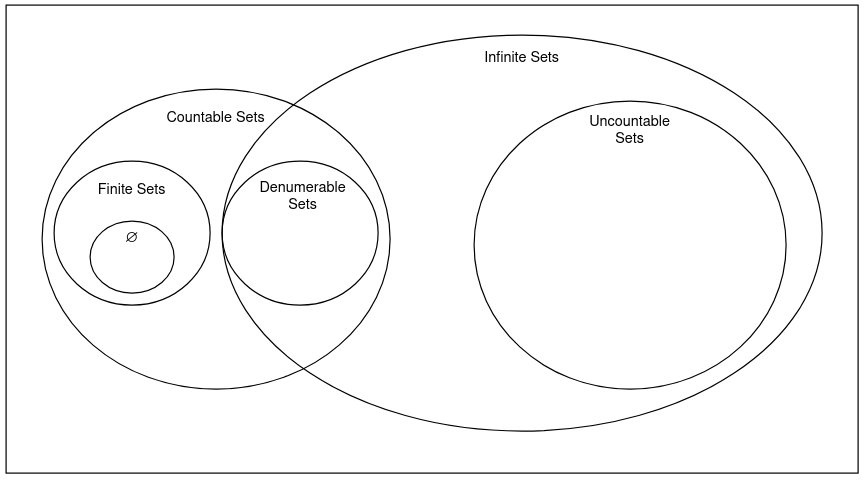
\includegraphics[width=\linewidth]{./imgs/Sets-Diagram.png}
	\caption{Venn Diagram representing the different kinds of sets.}
\end{figure}

\end{document}
